ในปัจจุบันมีชุดข้อมูลมากมายถูกสร้างขึ้นมาสำหรับใช้สร้างโมเดลสำหรับแก้ปัญหาในด้านต่างๆ เช่น การตรวจจับวัตถุภายในรูปภาพ
การจดจำใบหน้าบุคคลภายในรูปภาพ การจำแนกการกระทำของมนุษย์ เป็นต้น ซึ่งสิ่งที่ทำให้โมเดลปัญญาประดิษฐ์นั้นมีประสิทธิภาพสูงคือ
จำนวนของข้อมูล โดยในปัจจุบันปัญหาด้านการทำความเข้าใจรูปด้วยปัญญาประดิษฐ์ (image understanding) 
สามารถพัฒนาให้มีประสิทธิภาพสูงนั้นเนื่องจากมีจำนวนข้อมูลที่มากมาย ในขณะที่ปัญหาด้านการทำความเข้าใจวิดีโอด้วยปัญญาประดิษฐ์ (video understanding) 
นั้นกำลังมีการให้ความสนใจเพิ่มขึ้นเรื่อยๆในช่วงระยะเวลาหลายปีที่ผ่านมาในหัวข้อนี้จึงจะพูดถึงการศึกษาชุดข้อมูลที่ใช้สำหรับการทำความเข้าใจวิดีโอ 
โดยจะมุ่งเน้นไปที่การจำแนกการกระทำของมนุษย์เป็นหลัก

\subsection*{ชุดข้อมูล YouTube-8M} 
\subsubsection*{Youtube-8M}
YouTube-8M คือชุดข้อมูลวิดีโอที่เป็น multi-label ที่มีจำนวนวิดีโอเยอะที่สุด ซึ่งมีจำนวนมากถึง 8 ล้านวิดีโอ(ในปี 2016) โดยมีจุดมุ่งหมายหลักในการอธิบายธีมหลักของวิดีโอด้วยคำสั้นๆ เช่น ถ้าวิดีโอนั้นเป็นวิดีโอที่มี มนุษย์กำลังปั่นจักรยานบนถนนดินกับหน้าผา ชุดข้อมูลนี้จะอธิบายวิดีโอนี้ว่า mountain biking ซึ่งทำให้ YouTube-8M แตกต่างจากชุดข้อมูลวิดีโออื่นๆส่วนใหญ่ที่จะเน้น action หรือ activity ของมนุษย์ ซึ่งข้อมูลเชิงสถิติจะเป็นดังตารางที่ 1

\begin{figure}[!ht]
	\centering
	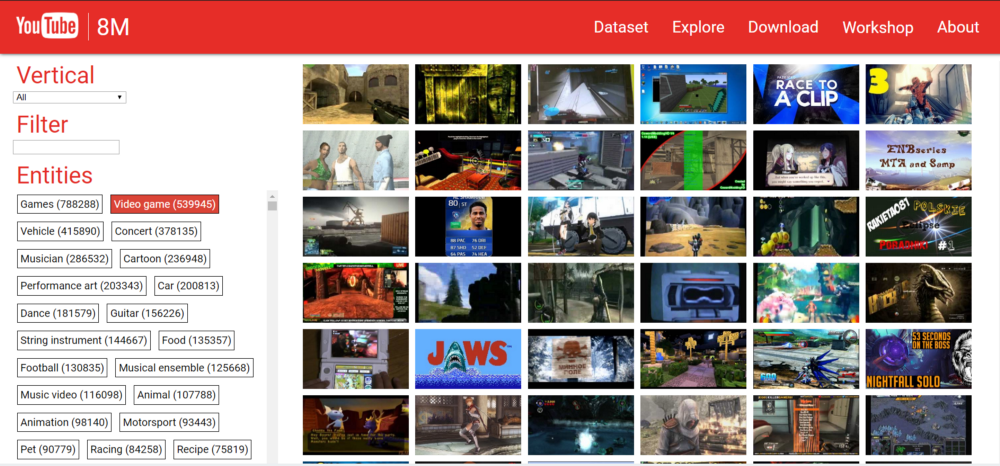
\includegraphics[width=1\textwidth]{chapter2/images/youtube-8m.png}
		\caption{ตัวอย่าง catagories ต่างๆของ YouTube-8M}
    	\label{fig:youtube-8m}
\end{figure}

\begin{table}[!ht]
\begin{tabular}{|c|c|c|c|c|}
		\hline
		{จำนวนวิดีโอ}&{ความยาวโดยรวมของวิดีโอ(ชม.)}&{จำนวนคลาสของวิดีโอ}&{ความยาวเฉลี่ยของแต่ละวิดีโอ(วินาที)}&{(จำนวนคลาสเฉลี่ยในแต่ละวิดีโอ)}\\
		\hline
		8,264,650			& ~500,000		& 4800		& 229.6		& 1.8											\\
		\hline
	\end{tabular}
	\caption{ข้อมูลเชิงสถิติของ YouTube-8M}
	\label{tab: ข้อมูลเชิงสถิติของ YouTube-8M}
\end{table}

\subsubsection*{1. วิธีการรวบรวมข้อมูล}
การเก็บข้อมูลของ YouTube-8M นั้นใช้เครื่องมือที่ชื่อว่า YouTube annotation system ในการเก็บรวบรวมข้อมูลโดยอาศัยผังความรู้(knowledge graph)ของ Google ในการค้นหาและรวบรวมข้อมูลในฐานข้อมูลของ YouTube
\begin{enumerate}
	\setlength\itemsep{-0.25em}
	\item กฏในการรวบรวมข้อมูลดังนี้
	\begin{enumerate}
		\setlength\itemsep{-0.25em}
		\item ทุกๆ หัวข้อต้องเป็นรูปธรรม
		\item ในแต่ละหัวข้อต้องมีจำนวนวิดีโอไม่น้อยกว่า 200 วิดีโอ
		\item ความยาวของวิดีโอต้องอยู่ระหว่าง 120 - 500 วินาที
	\end{enumerate}
หลังจากได้กฏในการรวบรวมข้อมูลแล้ว ขั้นตอนต่อไปคือการสร้างคำศัพท์(vocabulary)ที่ใช้ในการค้นหาข้อมูลวิดีโอจากใน YouTube 
	\item ขั้นตอนในการสร้างคำศัพท์มีดังนี้
	\begin{enumerate}
		\setlength\itemsep{-0.25em}
		\item กำหนด whitelist หัวข้อที่เป็นรูปธรรมมา 25 ชนิด เช่น game เป็นต้น
		\item กำหนด blacklist หัวข้อที่คิดว่าไม่เป็นรูปธรรมไว้ เช่น software เป็นต้น
		\item รวบรวมหัวข้อที่มีอยู่ใน whitelist อย่างน้อย 1 หัวข้อ และต้องไม่มีอยู่ใน blacklist ซึ่งจะทำให้ได้หัวข้อที่ต้องการมาประมาณ 50,000 หัวข้อ
		\item จากนั้นใช้ผู้ประเมินจำนวน 3 คน ในการคัดหัวข้อที่คิดว่าเป็นรูปธรรม และสามารถจดจำหรือเข้าใจได้ง่ายโดยไม่ต้องเชี่ยวชาญในด้านนั้นๆ ซึ่งผู้ประเมิน ก็จะมีคำถามว่า “ มันยากขนาดไหนถึงจะระบุได้ว่ามีหัวข้อดังกล่าวอยู่ในรูปหรือวิดีโอ โดยใช้เพียงแค่การมองรูปภาพเท่านั้น? ” โดยแบ่งเป็นระดับดังนี้
		\begin{enumerate}
			\setlength\itemsep{-0.25em}
			\item บุคคลทั่วไปสามารถเข้าใจได้
			\item บุคคลทั่วไปที่ผ่านการอ่านบทความที่เกี่ยวข้องมาแล้วสามารถเข้าใจได้
			\item ต้องเชี่ยญในด้านใดซักด้านจึงจะเข้าใจได้
			\item เป็นไปไม่ได้ ถ้าไม่มีความรู้ที่ไม่ได้เป็นรูปธรรม
			\item ไม่เป็นรูปธรรม
		\end{enumerate}
		\item หลังจากคำถามข้างบนและการให้คะแนน จะทำการเก็บไว้เฉพาะหัวข้อที่มีคะแนนเฉลี่ยมากที่สุดอยู่ที่ประมาณ 2.5 คะแนนเท่านั้น
		\item ทำให้สุดท้ายเหลือเพียงประมาณ 10,000 หัวข้อที่สามารถใช้ได้
		\item หลังจากได้หัวข้อที่คิดว่าเป็นรูปธรรมแล้วก็นำไปค้นหาและรวบรวมด้วย YouTube annotation system โดยมีขั้นตอนดังนี้
		\begin{enumerate}
			\setlength\itemsep{-0.25em}
			\item สุ่มเลือกวิดีโอมา 10 ล้านวิดีโอ พร้อมกับหัวข้อของวิดีโอ โดยใช้กฏที่กำหนดไว้ เอาหัวข้อที่มีจำนวนวิดีโอน้อยกว่า 200 วิดีโอออก
			\item ทำให้เหลือจำนวนวิดีโออยู่ 8,264,650 วิดีโอ
			\item แยกออกเป็น 3 ส่วน Train set, Validate set และ Test set ในอัตราส่วน 70:20:10 ตามลำดับ
		\end{enumerate}
	\end{enumerate}
\end{enumerate}

เนื่องจากชุดข้อมูลนี้มีขนาดมากกว่า 100 Terabytes และมีความยาวรวมประมาณ 500,000 ชั่วโมง ทำให้การจะใช้คอมพิวเตอร์ทั่วไปเปิดอาจจะใช้เวลานานถึง 50 ปี ทำให้ Google ทำการลดขนาดของข้อมูลลงโดยมีขั้นตอนดังนี้
\begin{figure}[!ht]
	\centering
	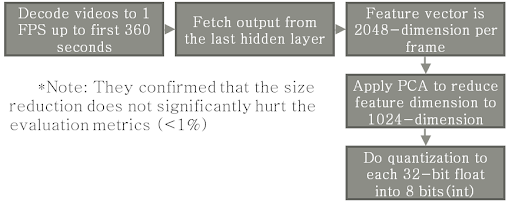
\includegraphics[width=1\textwidth]{chapter2/images/decrease_data.png}
		\caption{ขั้นตอนกระบวนการการลดขนาดของชุดข้อมูลให้สามารถใช้งานได้ง่ายยิ่งขึ้น}
    	\label{fig:decrease_data}
\end{figure}




\subsubsection*{2. การทดลองและวิเคราะห์ผล}
ในบทความ \footnote{YouTube-8M,https://arxiv.org/pdf/1609.08675.pdf} นั้นได้นำเสนอวิธีการในการจัดการข้อมูลซึ่งแบ่งเป็น 2 รูปแบบตามลักษณะของข้อมูลที่ใช้ และอัลกอริทึมหรือเทคนิคที่ใช้ในการสร้างโมเดล ดังนี้
\begin{enumerate}
	\setlength\itemsep{-0.25em}
	\item คุณลักษณะระดับเฟรม (Frame-level feature)
	\begin{enumerate}
		\setlength\itemsep{-0.25em}
		\item Frame-Level Models and Average Pooling
		\\ อันดับแรกเนื่องจากว่าชุดข้อมูลนี้ไม่มีการระบุหัวข้อในระดับเฟรม จึงใช้วิธีการนำหัวข้อในระดับวิดีโอ มากำหนดให้กับทุกๆเฟรมในวิดีโอแทน จากนั้นสุ่มเฟรมมา 20 เฟรมในแต่ละวิดีโอ ทำให้มีเฟรมถึง 120 ล้านเฟรม ซึ่งในแต่ละหัวข้อ $e$ ทำให้มี $(x_{i}, y_{i}^{e})$ 120 ล้านคู่ โดยที่ $x_{i} \epsilon  R^{1024}$ คือ คุณลักษณะที่ได้มาจาก hidden layer สุดท้ายก่อนจะเป็น fully connected และ $y_{i}^{e} \epsilon  0,1$ คือหัวข้อสำหรับหัวข้อ $e$ ของตัวอย่างที่ $i^{th}$ แล้วสร้างโมเดลทั้งหมด 4,800 โมเดลที่เป็นโมเดลแบบ one vs all classifier และเป็นอิสระต่อกันสำหรับแต่ละหัวข้อ และเนื่องจากการประเมินผลนั้นมีพื้นฐานมาจากหัวข้อในระดับวิดีโอ ทำให้ต้องทำการรวมความน่าจะเป็นของแต่ละหัวข้อในระดับเฟรมไปเป็นความน่าจะเป็นในระดับวิดีโอ โดยใช้การเฉลี่ยค่าความน่าจะเป็นทั้งหมดในหัวข้อนั้นๆ และใช้ average pooling เพื่อลดผลจากการตรวจจับความผิดปกติและความโดดเด่นของข้อมูลของแต่ละหัวข้อภายในวิดีโอ
		\clearpage
		\item Deep Bag of Frames (DBoF) Pooling
		\begin{figure}[!ht]
			\centering
			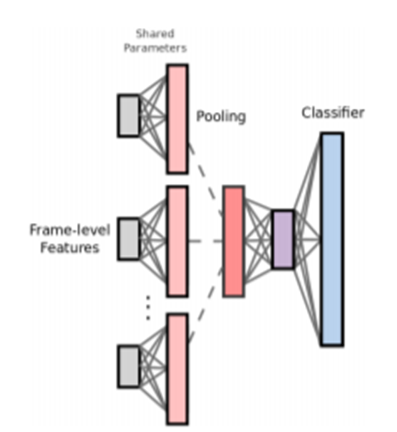
\includegraphics[width=0.5\textwidth]{chapter2/images/DBoF.png}
				\caption{โครงสร้างของโมเดล DBoF}
    			\label{fig:DBoF}
		\end{figure}
		\\ หลักการคล้ายๆกับ Deep Bag of Words โดยที่จะสุ่มเฟรม มา k เฟรม โดยที่แต่ละเฟรมเป็น N dimension input มาผ่าน fully connected ที่มี M units (M > N) และใช้ RELU activations แล้วทำ batch normalization ก่อนจะนำมารวมด้วย max pooling โดยที่ทั้งโครงข่ายใช้ Stochastic  Gradient Descent(SGD) 
		\item Long short-term memory(LSTM)
		\\ ในบทความ \footnote{YouTube-8M,https://arxiv.org/pdf/1609.08675.pdf} นี้ได้ใช้ LSTM แบบเดียวกับของ Beyond Short Snippets: Deep Networks for Video Classification \footnote{AVA,https://arxiv.org/pdf/1705.08421.pdf} แต่เนื่องจาก YouTube-8M นั้นผ่านการทำ preprocess มาแล้วทำให้ไม่สามารถใช้ raw video frame ได้ จึงทำได้เฉพาะ LSTM และ softmax layer เท่านั้น ตามรูปที่ \ref{fig:BSS}
		\begin{figure}[!ht]
			\centering
			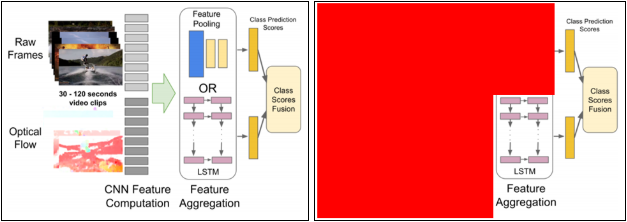
\includegraphics[width=1\textwidth]{chapter2/images/BSS.png}
				\caption{(ซ้าย) โครงสร้างจาก Beyond Short Snippets: Deep Networks for Video Classification, (ขวา) ส่วนที่สามารถใช้งานกับ YouTube-8M ได้}
    			\label{fig:BSS}
		\end{figure}
	\end{enumerate}
	\item คุณลักษณะระดับวิดีโอ (Video-level feature)
	\begin{enumerate}
		\setlength\itemsep{-0.25em}
		\item Video-level representation 
		\\ ในบทความ \footnote{YouTube-8M,https://arxiv.org/pdf/1609.08675.pdf}นี้ได้สำรวจวิธีการแยกเวกเตอร์คุณลักษณะระดับวิดีโอความยาวคงที่จากคุณลักษณะระดับเฟรมซึ่งการทำแบบนี้ทำให้ได้ประโยชน์ 3 ข้อ คือ 1) โมเดลทั่วไปที่ไม่ใช่ neural network สามารถนำไปใช้งานได้  2) ขนาดข้อมูลเล็กลง  3) เหมาะกับการนำไปสร้างโมเดล domain adaptive มากขึ้น
		\begin{enumerate}
			\setlength\itemsep{-0.25em}
			\item First, Second order and ordinal statistic
			\\ จากคุณลักษณะในระดับเฟรม $x_{1:F_{v}}^{v}$ โดยที่ $x_{j}^{v}$ คือคุณลักษณะระดับเฟรมในเฟรมที่ $j$ ของวิดีโอ $v$ และ $F_{v}$ คือจำนวนเฟรมทั้งหมดของวิดีโอ $v$ ทำการหาค่าเฉลี่ย $\mu_{v}$ และส่วนเบี่ยงเบนมาตรฐาน $\sigma_{v}$ พร้อมทั้งดึง ordinal statistics 5 อันดับแรกของแต่ละ dimension K ออกมา $Top_{k}(x^{v}(j)_{1:F_{v}})$ จะทำให้ได้เวคเตอร์คุณลักษณะ(feature-vector) $\varphi_{1:F_{v}}^{v}$ ของวิดีโอเป็นดังนี้ \\
			\centerline{$\varphi_{1:F_{v}}^{v} = \begin{bmatrix}
								\mu_{1:F_{v}}^{v}\\ 
								\sigma_{1:F_{v}}^{v}\\ 
								Top_{k}(x^{v}(j)_{1:F_{v}})
								\end{bmatrix}$}
			\item Feature normalization \\
			ก่อนที่จะทำการสร้าง one vs all classifiers แต่ละตัวนั้นได้ทำ normalization เวกเตอร์คุณลักษณะ $\varphi_{1:F_{v}}^{v}$ จากนั้นนำค่าเฉลี่ย $\mu_{v}$ ออกแล้วใช้ PCA ในการลด มิติของข้อมูล ซึ่งการทำแบบนี้นั้นทำให้การสร้างโมเดลเป็นไปได้เร็วขึ้น
		\end{enumerate}
		โดยการสร้างโมเดลด้วย video-level presentation นั้น บทความ \footnote{YouTube-8M,https://arxiv.org/pdf/1609.08675.pdf} นี้ได้หยิบมาทดสอบ 3 อัลกอริทึม
		\item Model training algorithm approaches 
		\begin{enumerate}
			\setlength\itemsep{-0.25em}
			\item Logistic Regression
			\item Hinge Loss
			\item Mixture of Experts (MoE)
		\end{enumerate}
		\item Evaluation metrics
		\begin{enumerate}
			\setlength\itemsep{-0.25em}
			\item Mean Average Precision (mAP)
			\item Hit@k
			\item Precision at equal recall rate (PERR)
		\end{enumerate}
	\end{enumerate}
	\item Results
	\begin{enumerate}
		\setlength\itemsep{-0.25em}
		\item Baseline on YouTube-8M dataset
\begin{table}[!ht]
\centering
\begin{tabular}{|c|c|c|c|c|}
		\hline
		{Inpute Features}&{Modeling Approach}&{mAP}&{Hit@1}&{(PERR)}\\
		\hline
		Frame-level, $(x_{1:F_{v}}^{v})$	& Logistic + Average		& 11.0		& 50.8		& 42.2					\\
		Frame-level, $(x_{1:F_{v}}^{v})$	& Deep Bag of Frames	& 26.9		& 62.7		& 55.1					\\
		Frame-level, $(x_{1:F_{v}}^{v})$	& LSTM				& 26.6		& 64.5		& 57.3					\\
		\hline
		Video-level, $\mu$					& Hinge loss					& 26.6		& 64.5		& 57.3				\\
		Video-level, $\mu$					& Logistic Regression				& 26.6		& 64.5		& 57.3				\\
		Video-level, $\mu$					& Mixture-of-2-Expert				& 26.6		& 64.5		& 57.3				\\
		Video-level, $\mu ; \sigma ; Top_{5} $	& Mixture-of-2-Expert				& 26.6		& 64.5		& 57.3				\\
		\hline
	\end{tabular}
	\caption{ประสิทธิภาพของโมเดลที่สร้างจาก YouTube-8M ด้วยวิธีต่างๆตามหัวข้อที่ 1 และ 2 โดยแถวที่ 1 คือ frame-level โมเดลและแถวที่ 2 คือ video-level โมเดล}
	\label{tab: ประสิทธิภาพของโมเดลที่สร้างจาก YouTube-8M}
\end{table}
\\
		จากตารางที่ \ref{tab: ประสิทธิภาพของโมเดลที่สร้างจาก YouTube-8M} จะเห็นว่าการทำ video-level features จากการหาค่าเฉลี่ยของ frame-level features แล้วสร้างโมเดลด้วย Hinge loss หรือ โมเดล Logistic Regression นั้นสามารถเพิ่มประสิทธิภาพได้ไม่น้อย และจากการทดลองทำให้เห็นว่า LSTM ที่มีความลึก 2 layers นั้นสามารถทำให้ผลลัพธ์เป็น state-of-the-art ในขณะนั้นได้ เนื่องจากในขณะที่ DBoF นั้นไม่ได้สนใจลำดับของเฟรม แต่ LSTM ใช้ state information เพื่อคงลำดับของเฟรมเอาไว้
\\
\\
		 LSTM นั้นดีที่สุดยกเว้น mAP, เนื่องจาก one-vs-all binary MoE classifier นั้นมีประสิทธิภาพดีกว่า, LSTM สามารถเพิ่มประสิทธิภาพบน Hit@1 และ PERR ได้เนื่องจากความสามารถในการเรียนรู้ความสัมพันธ์ระยะยาวในโดเมนของเวลา
		\clearpage
		\item Transfer learning video-level presentation from YouTube-8M to Sports-1M dataset
\begin{table}[!ht]
\centering
\begin{tabular}{|c|c|c|c|}
		\hline
		{Approach}&{mAP}&{Hit@1}&{(Hit@1)}\\
		\hline
		Logistic Regression ($\mu$)					& 58.0		& 60.1		& 79.6					\\
		Mixture-of-2-Expert ($\mu$)					& 59.1		& 61.5		& 80.4					\\
		Mixture-of-2-Expert ([$\mu ; \sigma ; Top_{5}$		& 61.3		& 63.2		& 82.6					\\
		LSTM									& 66.7		& 64.9		& 85.6					\\
		+Pretrained on YT-8M							& 67.6		& 65.7		& 86.2					\\
		\hline
		Hierarchical 3D Convolution						& -			& 61.0		& 80.0					\\
		Stacked 3D Convolutions						& -			& 61.0		& 85.0					\\
		LSTM with Optical Flow and Pixels				& -			& 73.0		& 91.0					\\
		\hline
	\end{tabular}
	\caption{ประสิทธิภาพของโมเดลเมื่อถูก transfer learning ด้วยชุดข้อมูล Sports-1M โดยใช้ video-level presentation}
	\label{tab: transfer learning}
\end{table}
\\
		จากตารางที่  \ref{tab: transfer learning} จะเห็นว่าโมเดล LSTM ที่ถูก pretrained จาก YouTube-8M นั้นมีประสิทธิภาพที่ดีกว่า ยกเว้น LSTM with Optical Flow and Pixels ที่มีการใช้ข้อมูลการเคลื่อนไหว(optical flow) ในการสร้างโมเดลด้วย
\\

		\item Transfer learning video-level presentation from YouTube-8M to ActivityNet dataset
\begin{table}[!ht]
\centering
\begin{tabular}{|c|c|c|c|}
		\hline
		{Approach}&{mAP}&{Hit@1}&{(Hit@1)}\\
		\hline
		Mixture-of-2-Expert ($\mu$)					& 69.1		& 68.7		& 85.4					\\
		+Pretrained PCA on YT-8M						& 74.1		& 72.5		& 89.3					\\
		Mixture-of-2-Expert ([$\mu ; \sigma ; Top_{5}$		& NO			& 74.2		& 72.3					\\
		+Pretrained PCA on YT-8M						& 77.6		& 74.9		& 91.6					\\
		LSTM									& 57.9		& 63.4		& 81.0					\\
		+Pretrained on YT-8M							& 75.6		& 74.2		& 92.4					\\
		\hline
		Ma, Bargal et al.								& 53.8		& -			& -						\\
		Heilbron et al.								& 43.0		& -			& -						\\
		\hline
	\end{tabular}
	\caption{ประสิทธิภาพของโมเดลเมื่อถูก transfer learning ด้วยชุดข้อมูล ActivityNet โดยใช้ video-level presentation}
	\label{tab: transfer learning ActivityNet}
\end{table}
\\
		จากตารางที่ \ref{tab: transfer learning ActivityNet} จะเห็นว่าโมเดลที่ถูก pretrained จาก YouTube-8M นั้นมีประสิทธิภาพที่ดีขึ้นมากเมื่อเทียบกับ benchmark ก่อนหน้า
	\end{enumerate}
\end{enumerate}

\subsubsection*{3. ปัญหาที่พบ}
เนื่องจากว่า YouTube-8M นั้นมีจำนวนข้อมูลที่เยอะมาก ทำให้ไม่สามารถตรวจสอบได้ทั้งหมดว่า ground-truth ของแต่ละวิดีโอนั้นมีความถูกต้องมากน้อยขนาดไหน ทำให้อาจเกิดข้อผิดพลาดได้ (ปัจจุบัน ปี 2019 YouTube-8M ได้มีการตรวจสอบข้อมูลอีกครั้ง เพื่อเพิ่มประสิทธิภาพของชุดข้อมูลซึ่งทำให้ปัจจุบันจำนวนข้อมูล และจำนวน category นั้นจะลดน้อยลงจากข้อมูลที่ใช้อ้างอิงในบทความ \footnote{YouTube-8M,https://arxiv.org/pdf/1609.08675.pdf} ข้างต้นที่ได้กล่าวมา)







%%%%%%%%%%%%%%%%%%%%%%%%%%%%%%%%%%%%%%%%%%%%%%%%%%%%%%%%%%%%%%%%%%%%%%%%%%%%%
\clearpage
\subsection*{ชุดข้อมูล Atomic visual action (AVA)}	
AVA\textsuperscript{\cite{AVA}} คือ ชุดข้อมูลที่รวบรวมวิดิโอที่มีความยาว 15 นาที ถูกแบ่งด้วยความถี่ 1 hz (900 keyframes) จากในภาพยนต์โดยยึดการกระทำของมนุษย์เป็นศูนย์กลาง
เพื่อใช้สำหรับสร้างโมเดลที่เข้าใจกิจกรรมของมนุษย์ในวิดิโอว่ามนุษย์กำลังทำอะไรอยู่ ซึ่งข้อดีของ AVA คือ ชุดข้อมูลจะมีคำกำกับเป็นแบบทวิคำกำกับ (multiple label)
และคำกำกับของ AVA มีจำนวน 80 ประเภท สามารถแบ่งได้เป็นสามหมวดหมู่คือ ท่าทาง (Pose), ปฏิสัมพันธ์กับวัตถุ (Interaction with object) 
และปฏิสัมพันธ์กับบุคคล (Interaction with people) ซึ่งสามารถมีคำกำกับได้มากสูงสุดถึง 7 คำกำกับ
\begin{enumerate}
	\item {รายละเอียดชุดข้อมูล}
	\begin{enumerate}
		\item ขั้นตอนการเก็บข้อมูลสำหรับการทำชุดข้อมูลมีขั้นตอนการทำ 5 ขั้นดังนี้
		\begin{enumerate}
			\item การสร้างคำศัพท์การกระทำจะมีหลักการ 3 ข้อในการรวบรวมคำศัพท์ดังนี้
			\begin{enumerate}
				\item เก็บรวบรวมคำศัพท์ทั่วไปที่เกิดขึ้นในชีวิตประจำวัน
				\item จะต้องมีเอกลักษณ์สามารถเห็นได้ชัดเจน เช่น การถือของ
				\item กำหนดรูปแบบของคำศัพท์ขึ้นมา และใช้ความรู้จากชุดข้อมูลอื่นในการทำให้ได้หมวดหมู่การกระทำของมนุษย์ที่ครอบคลุม
			\end{enumerate}
			\item ภาพยนต์และส่วนที่เลือกมาใช้ทำชุดข้อมูล AVA ทั้งหมดจะถูกนำมาจาก YouTube โดยเริ่มจากการรวบรวมเอารายชื่อของนักแสดงที่มีชื่อเสียง
			ซึ่งจะมีความหลากหลายของเชื้อชาติรวมกันอยู่ วิดีโอที่ถูกคัดเลือกจะมีเกณฑ์ดังนี้
			\begin{enumerate}
				\item วิดีโอต้องอยู่ในหมวด ภาพยนต์ และละครโทรทัศน์
				\item วิดีโอจะต้องมีความยาวมากกว่า 30 นาที
				\item เผยแพร่มาแล้วเป็นระยะเวลาอย่างน้อย 1 ปี
				\item มีจำนวนยอดคนดูมากกว่า 1,000 ครั้ง
				\item ละเว้นวิดีโอบางประเภท เป็นภาพขาว-ดำ มีความละเอียดต่ำ การ์ตูน หรือวิดีโอเกม
			\end{enumerate}
			\item การสร้างกรอบสี่เหลี่ยมครอบมนุษย์ที่อยู่ภายในภาพประกอบด้วย 2 ขั้นตอน
			\begin{enumerate}
				\item สร้างกรอบสี่เหลี่ยมโดยใช้โมเดลปัญญาประดิษฐ์ faster RCNN สำหรับการตรวจจับมนุษย์
				\item ใช้มนุษย์ในการตรวจสอบและแก้ไขกรอบสี่เหลี่ยมที่ผิดพลาด
			\end{enumerate}	
			\item การติดตามตำแหน่งของบุคคล\\
			ทำการติดตามตำแหน่งของบุคคลที่อยู่ในช่วงเวลาเดียวกันด้วยใช้วิธีการแทร็กโดยยึดมนุษย์เป็นศูนย์กลาง โดยการคำนวณค่าความใกล้เคียงกันระหว่างบุคคล 
			โดยใช้ person embedding (ใช้โครงข่ายประสาทเทียมในการหาฟีเจอร์ขั้นสูงและใช้เมทริกซ์ในการหาความสัมพันธ์ของแต่ละคน) จากนั้นจะใช้อัลกอริทึม Hungarian distance (อัลกอริทึ่มสำหรับการหาข้อเสนอที่ดีที่สุด) ในการหาตัวเลือกคู่ของกรอบสี่เหลี่ยมที่ดีที่สุด
			\item การสร้างคำกำกับคุณลักษณะ\\
			การสร้างคำกำกับของการกระทำจะถูกสร้างขึ้นโดยมนุษย์ ซึ่งผู้วิจัยจะใช้โปรแกรมสำหรับช่วยเหลือในการสร้างคำกำกับคุณลักษณะ โดยสามารถกำหนดคำกำกับของการกระทำได้สูงสุดถึง 7 คำต่อ 1 กรอบสี่เหลี่ยม นอกจากนั้นสามารถตั้งสถานะเนื้อหาที่ไม่เหมาะสม หรือ กรอบสี่เหลี่ยมที่ผิดพลาดได้อีกด้วย ซึ่งในทางปฎิบัติเพื่อลดโอกาสที่จะเกิดข้อผิดพลาด จึงแบ่งขั้นตอนในการสร้างคำกำกับออกเป็น 2 ขั้นตอนดังนี้
			\begin{enumerate}
				\setlength\itemsep{-0.25em}
				\item สร้างข้อเสนอสำหรับคำกำกับของการกระทำ
				\item ข้อเสนอจะถูกตรวจสอบข้อเสนอที่ได้จากขั้นตอนแรก ซึ่งจะใช้มนุษย์ในการตรวจสอบ 3 คน โดยคำกำกับจะต้องถูกตรวจสอบด้วยผู้ตรวจสอบอย่างน้อย 2 คน จึงจะถูกยึดเป็นคำกำกับหลัก
			\end{enumerate}
		\end{enumerate}
	\end{enumerate}
	\item {โมเดลปัญญาประดิษฐ์}
	\begin{enumerate}
		\item โมเดลปัญญาประดิษฐ์ที่งานวิจัยนี้ใช้ คือ two stream variant ซึ่งจะทำการประมวลผลทั้ง RGB flow และ optical flow 
		โดยเป็นโครงสร้างของ faster RCNN ที่นำ Inception network เข้ามาใช้
		\item เครื่องมือที่ใช้วัดผลสำหรับงานวิจัยนี้ คือค่า IoU และ 3D IoUs 
		\begin{enumerate}
			\item ค่า IoU คือค่าที่ใช้วัดความสอดคล้องระหว่างสองกรอบสี่เหลี่ยม(กรอบสี่เหลี่ยมจริงของเฟรม และ กรอบสี่เหลี่ยมที่ทำนายขึ้นมา) ซึ่งใช้สำหรับการวัดผลระดับเฟรม 
			\item ค่า 3D IoUs คือค่าที่ใช้วัดความสอดคล้องระหว่างกรอบสี่เหลี่ยมภายใน 2 วิดีโอ ซึ่งใช้สำหรับการวัดผลระดับวิดีโอ โดยเทียบกันระหว่างกรอบสี่เหลี่ยมจริงในช่วงของเฟรมที่ต่อกัน (ground-truth tubes) และ กรอบสี่เหลี่ยมที่ทำนายขึ้นมาในช่วงของเฟรมที่ต่อกัน (linked detection tubes) 
		\end{enumerate}
		\item ประสิทธิภาพของโมเดลปัญญาประดิษฐ์ในปัจจุบัน
		\\ข้อมูลโมเดลปัญญาประดิษฐ์ที่นำมาทดสอบ
		\begin{enumerate}				
			\item Actionness\textsuperscript{\cite{actioness}} เป็นการหาความน่าจะเป็นของการกระทำ โดยใช้โครงสร้างของ hybrid fully convolutional network (HFCN) hybrid fully เป็นโครงสร้างที่ประกอบด้วยโครงข่ายประสาทเทียม 2 ชนิด คือ
			\begin{enumerate}
				\item Appearance-FCN (A-FCN) คือ โครงข่ายประสาทเทียมที่นำมาใช้แสดงลักษณะของวัตถุ(ตำแหน่งวัตถุ, ความตื้นลึกวัตถุ) ที่ปรากฎบนรูป RGB1
				\item MotionFCN (M-FCN) คือ โครงข่ายประสาทเทียมที่แยกการเคลื่อนไหวจากข้อมูลของ optical flow
			 \end{enumerate}
			\item Peng without MR, Peng with MR (Multi-region two-stream R-CNN)\textsuperscript{\cite{peng}} เป็นโมเดลปัญญาประดิษฐ์ที่ใช้สำหรับตรวจจับวิดีโอในชีวิตจริง ซึ่งพื้นฐานของโมเดลนี้เป็น Faster R-CNN โดยโมเดลนี้มีกระบวนการ 3 กระบวนการคือ
			\begin{enumerate}
					\item สร้างข้อเสนอพื้นที่ที่มีการเคลื่อนไหว
					\item สะสม Optical flow จากเฟรมหลายๆเฟรม เพื่อนำไปปรับปรุงการตรวจจับการกระทำ
					\item นำพื้นที่หลายๆส่วนมาวิเคราะห์ผ่านโมเดล Faster R-CNN
			\end{enumerate}
			\item ACT Action Tubelet Detector\textsuperscript{\cite{act}} เป็นการระบุตำแหน่งของการกระทำที่มีระยะเวลาๆสั้นๆ ซึ่งใช้วิธีการตรวจจับระดับเฟรม และ ใช้การติดตามตำแหน่งในการเชื่อมระหว่างเฟรมปัจจุบันไปยังเฟรมถัดไป. ACT ถูกสร้างต่อจาก SSD framework และ ใช้คอนโวลูชันในการสกัดคุณลักษณะในแต่ละเฟรมซึ่งการคิดคะแนนและความน่าจะเป็นของหมวดหมู่จะคิดจากการนำคุณลักษณะเรียงต่อกัน และ หาข้อมูลจากลำดับข้อมูลนั้น
		\end{enumerate}
		จากการทดสอบการเทียบโมเดลปัญญาประดิษฐ์ของงานวิจัยนี้และวิธีการอื่นๆ โดยนำไปทดสอบกับชุดข้อมูลวิดีโอ JHMDB และ UCF101-24 ได้ผลลัพธ์ออกมาดังนี้
			\begin{table}[!ht]
				\centering
				\begin{tabular}{|c|c|c|c|}
					\hline
					{Frame-mAP}&{JHMDB (mAP)}&{UCF101-24 (mAP)}								\\
					\hline
					Actionness 			& 39.9				& 	-						\\
					Peng w/o MR			& 56.9				& 64.8						\\
					Peng w/  MR 			& 58.5				& 65.7						\\
					ACT					& 65.7				& 69.5						\\
					\hline
					2 stream(Our approach)		& \textbf{73.3}		& \textbf{76.3}				\\
					\hline
				\end{tabular}
				\caption{ผลการทดลองของวิธีต่างๆบนคุณลักษณะระดับเฟรม}
				\label{tab: transfer learning}
			\end{table}
		\item ปัญหาที่พบ
		ในปัจจุบันยังไม่มีโมเดลปัญญาประดิษฐ์ที่ทดสอบด้วยชุดข้อมูล AVA และได้ผลการทำงานที่ดี เนื่องจากชุดข้อมูลนี้สนใจการกระทำของมนุษย์ที่มีรายละเอียดเล็กๆน้อยๆ 
		ทำให้ยากต่อการทำนายสำหรับโมเดลปัญญาประดิษฐ์
	\end{enumerate}
\end{enumerate}
%%%%%%%%%%%%%%%%%%%%%%%%%%%%%%%%%%%%%%%%%%%%%%%%%%%%%%%%%%%%%%%%%%%%%%%%%%%%%
\clearpage
\subsubsection*{ชุดข้อมูล Moments in Time}
Moments in time\textsuperscript{\cite{monfort2019moments}} คือชุดข้อมูลที่ใช้มนุษย์ในการกำกับข้อมูลทั้งหมดให้กับวิดีโอสั้นถึง 1 ล้านวิดีโอ 
และมีจำนวนกิจกรรมหรือการกระทำต่างกัน 339 หมวดหมู่ โดยแต่ละวิดีโอจะมีความยาวอยู่ที่ 3 วินาที เนื่องจากเป็นเวลาเฉลี่ยที่มนุษย์ใช้ในการเข้าใจกับเหตุการณ์ที่เกิดขึ้น
(human working memory) รูปแบบของชุดข้อมูลจะมีอยู่ทั้งหมดอยู่ 3 รูปแบบ ได้แก่ ภาพนิ่ง (spatial) เสียง (auditory) และการเคลื่อนไหว (temporal) 
นอกจากนี้ชุดข้อมูลนี้นั้นไม่รวบรวมเพียงแค่การกระทำของมนุษย์เท่านั้น ยังรวมไปถึง สัตว์ สิ่งของ และปรากฏการณ์ธรรมชาติ ทำให้ชุดข้อมูลนี่เป็นการท้าทายรูปแบบใหม่เพราะด้วยข้อมูลที่มีความซับซ้อนมากขึ้น
\begin{enumerate}
	\item {รายละเอียดชุดข้อมูล}
	\begin{enumerate}
		\setlength\itemsep{-0.25em}
		\item เป้าหมายของชุดข้อมูล : สนใจเหตุการณ์ที่เกิดขึ้นในวิดีโอ เช่น การกระทำของคนหรือสัตว์ เหตุการณ์ และปรากฎการณ์ธรรมชาติ 
		\item จำนวนของวิดีโอ : มากกว่า 1,000,000 วิดีโอ
		\item ความยาวเฉลี่ยของแต่ละวิดีโอ : 3 วินาที
		\item จำนวนของหมวดหมู่ : 339 หมวดหมู่
		\item วิธีการเก็บรวบรวมข้อมูล
	\begin{enumerate}
		\item เริ่มจากการรวบรวมคำที่ใช้อยู่ทั่วไปในชีวิตประจำวันมา 4,500 คำจาก VerbNet\textsuperscript{\cite{Schuler:2005:VBC:1104493}} เว็บไซต์ที่เก็บรวบรวมคำกิริยาภาษาอังกฤษขนาดใหญ่ 
		จากนั้นนำมาแบ่งกลุ่มคำที่มีความหมายใกล้เคียงกันโดยใช้คุณลักษณะจาก Propbank\textsuperscript{\cite{Zaghouani:2010:RAP:1868720.1868756}} และ
		FrameNet\textsuperscript{\cite{Baker:1998:BFP:980451.980860}} โดยเก็บข้อมูลเป็นแบบเวกเตอร์คุณลักษณะฐานสอง (binary feature vector) 
		ซึ่งถ้าคำใดมีความเกี่ยวข้องกันทางคุณลักษณะก็จะให้ค่าเป็น 1 ถ้าไม่เกี่ยวข้องกันจะให้ค่าเป็น 0 จากนั้นจึงใช้วิธี k-means clustering ในการแบ่งกลุ่ม 
		เมื่อแบ่งกลุ่มแล้วจากนั้นจะเลือกคำจากในแต่ละกลุ่มนั้น โดยคำที่เลือกมานั้นจะเป็นคำที่ใช้บ่อยที่สุดในกลุ่มนั้น และลบคำนั้นออกจากกลุ่มอื่นๆทั้งหมด (คำๆหนึ่งสามารถอยู่ได้หลายกลุ่ม) 
		จากนั้นจะทำกระบวนการนี่ไปเรื่อยๆ แต่คำที่เลือกมาจะต้องไม่มีความหมายคลุมเครือ หรือเป็นสิ่งที่ไม่สามารถมองเห็นหรือได้ยินได้ และต้องไม่มีความหมายเหมือนกับคำที่เคยเลือกมาก่อน 
		จนสุดท้ายแล้วได้ออกมาที่ 339 หมวดหมู่
		\item ต่อมาทำการหาชุดข้อมูลวิดีโอโดยจะตัดออกมาเพียง 3 วินาทีที่เกี่ยวข้องกับคำใน 339 หมวดหมู่ที่เลือกมาจากวิดีโอแหล่งต่างกัน 10 แหล่ง 
		การตัดวิดีโอนั้นจะไม่ใช้พวก Video2Gif (โมเดลที่ระบุตำแหน่งของสิ่งที่น่าสนใจในวิดีโอ) เพราะจะทำให้เกิดอคติขึ้นจะเกิดขึ้นตอนสร้างโมเดล ดังนั้นจึงใช้มนุษย์ในการตัดวิดีโอ จากนั้นจะทำการส่งข้อมูลของคำ
		และวิดีโอที่ตัดไปยัง Amazon Mechanical Turk (AMT หรือตลาดแรงงาน) เพื่อทำการสร้างคำกำกับโดยพนักงานของ AMT ทำให้ได้ 64 วิดีโอที่เกี่ยวข้องกับคำหนึ่ง 
		และอีก 10 วิดีโอที่มีคำกำกับอยู่แล้ว โดยวิดีโอที่มีคำกำกับอยู่แล้วนั้นถ้าพนักงานของ AMT ตอบเหมือนกันเกิน 90\% ถึงจะนำเข้าไปรวมกับชุดข้อมูลส่วนอีก 64 วิดีโอ
		ถ้าเป็นชุดข้อมูลสำหรับสร้างโมเดลจะต้องผ่านพนักงานของ AMT อย่างน้อย 3 ครั้ง และต้องมีคำกำกับเหมือนกัน 75\% ขึ้นไปถึงจะถือว่าเป็นคำกำกับที่ถูกต้อง 
		ถ้าเป็นชุดข้อมูลสำหรับตรวจคำตอบ และชุดข้อมูลสำหรับทดสอบจะต้องผ่านพนักงานของ AMT อย่างน้อย 4 ครั้ง และต้องมีคำกำกับเหมือนกัน 85\% ขึ้นไป 
		เหตุผลที่ไม่ตั้งเกณฑ์ไว้ที่ 100\% เพราะจะทำให้วิดีโอนั้นยากเกินไปที่จะทำให้สามารถจำการกระทำได้	
	\end{enumerate}
\end{enumerate}
	\item การเตรียมข้อมูล
		\begin{enumerate}
			\item ชุดข้อมูลสำหรับสร้างโมเดลจะมี 802,264 วิดีโอ และมีวิดีโอในแต่ละหมวดหมู่อยู่ที่ 500 ถึง 5,000 วิดีโอ
			\item ชุดข้อมูลสำหรับตรวจคำตอบจะมี 33,900 วิดีโอ และมีวิดีโอในแต่ละหมวดหมู่อยู่ที่ 100 วิดีโอ
			\item แยกเฟรม RGB ออกมาจากวิดีโอ และทำการเปลี่ยนขนาดให้เป็น 340\texttimes256  pixel
			\item ใช้อัลกอริทึม TVL1 optical flow จาก Opencv เพื่อลดข้อมูลรบกวนที่จะเกิดขึ้น
			\item ทำการแปลงค่าที่อยู่ใน optical flow ให้เป็นเลขจำนวนเต็มเพื่อทำให้การคำนวณนั้นเร็วยิ่งขึ้น
			\item ปรับค่า displacement ใน optical flow ให้ค่าสูงสุดเป็น 15 ต่ำสุดเป็น 0 และทำการปรับขนาดให้เป็นช่วง 0 - 255
			\item เก็บข้อมูลออกมาในรูปแบบของภาพขาวดำเพื่อลดพื้นที่ในการเก็บข้อมูล
			\item แก้ปัญหาเรื่องการเคลื่อนไหวของกล้องด้วยการนำค่าเฉลี่ยของเวกเตอร์ไปลบกับ displacement
			\item สุดท้ายจะเป็นสุ่มตัดภาพออกมาเพื่อเพิ่มจำนวนข้อมูล
		\end{enumerate}
	\item {โมเดลปัญญาประดิษฐ์}
	\begin{enumerate}
		\item ในงานวิจัยนี้มีการทดสอบโมเดลปัญญาประดิษฐ์หลายรูปแบบ โดยโมเดลปัญญาประดิษฐ์ที่มีประสิทธิภาพการทำงานที่ดีที่สุด 5 ลำดับแรกมีดังนี้
			\begin{enumerate}
				\item SVM มีรูปแบบข้อมูลที่ป้อนเข้า คือ เฟรมที่ต่อเนื่อง (spatial) + เฟรมเดี่ยว (temporal) + ข้อมูลเสียง (auditory) 	
				\item I3D มีรูปแบบข้อมูลที่ป้อนเข้า คือ เฟรมที่ต่อเนื่อง + เฟรมเดี่ยว
				\item TRN-Multiscale มีรูปแบบข้อมูลป้อนเข้า คือ เฟรมที่ต่อเนื่อง + เฟรมเดี่ยว
				\item TSN-2stream มีรูปแบบข้อมูลป้อนเข้า คือ เฟรมที่ต่อเนื่อง + เฟรมเดี่ยว
				\item ResNet50-ImageNet	มีรูปแบบข้อมูลป้อนเข้า คือ เฟรมที่ต่อเนื่อง
			\end{enumerate}
		\item เครื่องมือที่ใช้วัดผลงานวิจัยนี้
			\begin{enumerate}
				\item Classification accuracy Top-1, Top-5
			\end{enumerate}
		\item ประสิทธิภาพของโมเดลปัญญาประดิษฐ์ในปัจจุบัน
			\begin{enumerate}
				\item ทำการทดสอบด้วยวิธี cross dataset transfer โดยการนำโมเดล ResNet50 I3D ที่สร้างด้วยชุดข้อมูล Kinetics และ Moments in Time 
				แล้วนำทั้ง 2 โมเดลไปทดสอบกับชุดข้อมูลอื่น โดยจะปรับอัตราความถี่ของเฟรม (frame rate) ของวิดีโอให้เป็น 5 fps
				\begin{table}[!ht]
					\centering
					\begin{tabular}{|c|c|c|c|}
						\hline
						{Pretrained}&\multicolumn{3}{c|}{Fine-Tuned}\\
						\cline{2-4}
						{}								& UCF-101			& HMDB-51			& Something Something			\\
						\hline
						\multirow{2}{*}{Kinetics}		& Top-1 : 92.6		& Top-1 : 62.0		& Top-1 : 48.6		\\
						{}								& Top-5 : 99.2		& Top-5 : 88.2		& Top-5 : 77.9		\\
						\hline
						\multirow{2}{*}{Moments}		& Top-1 : 91.9		& Top-1 : 65.9		& Top-1 : 50.0		\\
						{}								& Top-5 : 98.6		& Top-5 : 89.3		& Top-5 : 78.8		\\
						\hline
					\end{tabular}
					\caption{ประสิทธิภาพของโมเดล Resnet50 I3D ที่ใช้ชุดข้อมูล Kinetics และ Moments in Time}
					\label{tab: Data transfer performance ของโมเดล Resnet50 I3D}
				\end{table}
				\item จะเห็นได้ว่า Kinetics ให้ผลลัพธ์ที่ดีกว่าใน UCF-101 เพราะว่ามีหมวดหมู่ที่ตรงกันอยู่หลายอย่าง ในขณะที่ HMDB-51 นั้นมีการรวบรวมข้อมูลจากหลายแหล่ง 
				และมีจำนวนหมวดหมู่ที่หลากหลายจึงทำให้มีความใกล้เคียงกับตัวข้อมูลของ Moments in Time ดังนั้นจึงเทียบผลลัพท์จาก Something Something 
				ซึ่งจะทำให้เห็นว่า Moments in Time มีประสิทธิภาพที่ดีกว่าและวิดีโอที่มีความยาวมากกว่า 3 วินาทีจะไม่ส่งผลกระทบกับประสิทธิภาพของ Moments in Time
		\end{enumerate}
	\end{enumerate}
	\item {ปัญหาที่พบ}\\
	ผลลัพธ์จากการทำนายด้วยโมเดลถ้าผ่านภาพที่มีรายละเอียดเยอะจะทำให้การ ทำนายโอกาสผิดนั้นค่อนข้างสูง ซึ่งปัญหานี่สามารถทำให้เกิดน้อยลงด้วยการนำวิธี 
	class activation mapping (CAM) จะเป็นการเน้นภาพในส่วนที่มีข้อมูลมากที่สุดและทำนายผลออกมา แต่ก็ยังมีจุดที่เป็นปัญหาอยู่ เช่น 
	การกระทำที่เกิดขึ้นเร็วมากจะทำให้การทำนายนั้นมีโอกาสผิดสูงขึ้น
\end{enumerate}		